\appendix

\section*{Appendix}

\if0{
\section{Additional Notes on the Use of NLI}
\label{app:nli}

There are other tasks modeling relationships between sentences.
Paraphrase~\citep{paranmt} and semantic relatedness~\citep{semeval} tasks are such examples.
It is possible to automatically create large-scale paraphrase datasets by machine translation~\citep{ppdb}.
However, our task is not a paraphrasing task, and creating negative examples is crucial and non-trivial~\citep{selectional-preference}.
In contrast, as described above, the NLI setting comes with negative examples by nature.
This is not ideal for the intent detection task, because we need to discriminate between topically similar utterances of different intents.
In summary, the NLI task well matches our objective, with access to large datasets.
}\fi

\if0{
\section{A Note on the Threshold Selection} \label{threshold-selection}
\label{app:threshold}
Our joint score ($\mathrm{Acc}_\mathrm{in} + R_\mathrm{oos}$) in Section~4.2 gives the same weight to the two metrics, $\mathrm{Acc}_\mathrm{in}$ and $R_\mathrm{oos}$, compared to other combined metrics like $(C_\mathrm{in}+C_\mathrm{oos})/(N_\mathrm{in}+N_\mathrm{oos})$.
Such a combined metric can put much more weight on the in-domain accuracy when $N_\mathrm{in}$ and $N_\mathrm{oos}$ are imbalanced; Table~2 shows such imbalance on the development set.
\citet{oos-intent} sacrificed the OOS recall a lot, and the trade-off with respect to the threshold selection was not discussed.
}\fi


\begin{table*}[h]
\centering
%\resizebox{1.0\linewidth}{!}{
\begin{tabular}{l|lll}
\hline
Dataset                    & SNLI & WNLI & MNLI \\ \hline
Size of the development set & 9999          & 70            & 9814          \\
Accuracy                   & 94.5\%        & 41.4\%        & 92.1\%        \\ \hline
\end{tabular}\caption{Development results on three NLI datasets.}
\label{table-pretrain}
\end{table*}

\section{Training Details} \label{training-details}

\paragraph{Dataset preparation}
%To use the CLINC150 dataset~\citep{oos-intent}\footnote{\url{https://github.com/clinc/oos-eval}.} in our ways, especially for the single-domain experiments, we provide a zip file {\tt data\_preprocess\_for\_emnlp2020.zip} accompanied with the paper submission.
To use the CLINC150 dataset~\citep{oos-intent}\footnote{\url{https://github.com/clinc/oos-eval}.} in our ways, especially for the single-domain experiments, we provide preprocessing scrips accompanied with our code.

\paragraph{General training}\label{appendix-general-training}
This section describes the details about the model training in Section~\ref{subsec:model_setting}.
For each component related to RoBERTa and SRoBERTa, we solely follow the two libraries, transformers and sentence-transformers, for the sake of easy reproduction of our experiments.\footnote{\url{https://github.com/huggingface/transformers} and \url{https://github.com/UKPLab/sentence-transformers}.}
The example code to train the NLI-style models is also available.\footnote{\url{https://github.com/huggingface/transformers/tree/master/examples/text-classification}.}
We use the {\tt roberta-base} configuration\footnote{\url{https://s3.amazonaws.com/models.huggingface.co/bert/roberta-base-config.json}.} for all the RoBERTa/SRoBERTa-based models in our experiments.
All the model parameters including the RoBERTa parameters are updated during all the fine-tuning processes, where we use the AdamW~\citep{adamw} optimizer with a weight decay coefficient of 0.01 for all the non-bias parameters.
We use a gradient clipping technique~\citep{clip} with a clipping value of 1.0, and also use a linear warmup learning-rate scheduling with a proportion of 0.1 with respect to the maximum number of training epochs. 



\begin{table*}[t]
\centering
\resizebox{1.0\linewidth}{!}{
\begin{tabular}{l|ccc|ccc}
\hline
           & \multicolumn{3}{c|}{\textbf{Single domain}}                 & \multicolumn{3}{c}{\textbf{All domains}}                 \\ \cline{2-7} 
           & \textbf{Learning rate} & \textbf{Epoch}    & \textbf{Run} & \textbf{Learning rate} & \textbf{Epoch} & \textbf{Run} \\ \hline
Classifier & \{1e-4, 2e-5, 5e-5\}   & \{15, 25, 35\}    & 10             & \{1e-4, 5e-5\}         & \{15, 25, 35\} & 5              \\
Emb-kNN    & \{1e-4, 2e-5, 3e-5\}   & \{7, 10, 20, 25, 35\} & 10             &   \{2e-5, 5e-5\}        &  \{3, 5, 7\}        & 5              \\
DNNC       & \{1e-5, 2e-5, 3e-5, 4e-5\}   & \{7, 10, 15\}     & 10             & \{2e-5, 5e-5\}         & \{3, 5, 7\}   & 5              \\ \hline
\end{tabular}}\caption{Some hyper-parameter settings for a few models.}\label{table:hyper-paramter}
\end{table*}
%%%%%%%%%%%%%%%%%%%%%%%%%%%%%%%%%%%%%%%%%%%%%%%%%%%%%%%



%%%%%%%%%%%%%%%%%%%
\begin{table*}[t]
\centering
%\resizebox{0.8\linewidth}{!}{
\begin{tabular}{l|cc}
\hline
           & \textbf{5-shot}                 & \textbf{10-shot}                \\ \hline
Classifier & \{bs: 50, ep: 25.0, lr: 5e-05\} & \{bs: 50, ep: 35.0, lr: 5e-05\} \\ \hline
Emb-kNN    & \{bs: 200, ep: 7.0, lr: 2e-05\} & \{bs: 200, ep: 5.0, lr: 2e-05\}  \\ \hline
DNNC       & \{bs: 900, ep: 7.0, lr: 2e-05\} &  \{bs: 1800, ep: 5.0, lr: 2e-05\} \\ \hline
\end{tabular}
%}
\caption{Best hyper-parameter settings for a few models on the all-domain experiments, where {\tt bs} is batch size, {\tt ep} represents epochs, {\tt lr} is learning rate.}\label{table:hyper-paramter-best-all}
\end{table*}



\begin{table*}[t]
\centering
\resizebox{1.0\linewidth}{!}{
\begin{tabular}{l|cccc}
\hline
           & \textbf{5-shot}                                      & \multicolumn{1}{c|}{\textbf{10-shot}}                 & \textbf{5-shot}                  & \textbf{10-shot}                 \\ \cline{2-5} 
           & \multicolumn{2}{c|}{\textbf{Banking}}                                                                                 & \multicolumn{2}{c}{\textbf{Credit cards}}                                    \\ \hline
Classifier & \multicolumn{1}{l}{\{bs: 15, ep: 25.0, lr: 5e-05\}}  & \multicolumn{1}{l|}{\{bs: 15, ep: 35.0, lr: 5e-05\}}  & \{bs: 15, ep: 15.0, lr: 5e-05\}  & \{bs: 15, ep: 25.0, lr: 5e-05\}  \\
Emb-kNN    & \multicolumn{1}{l}{\{bs: 200, ep: 35.0, lr: 1e-05\}} & \multicolumn{1}{l|}{\{bs: 200, ep: 25.0, lr: 2e-05\}} & \{bs: 100, ep: 20.0, lr: 1e-05\} & \{bs: 100, ep: 10.0, lr: 1e-05\} \\
DNNC       & \multicolumn{1}{l}{\{bs: 370, ep: 15.0, lr: 1e-05\}} & \multicolumn{1}{l|}{\{bs: 370, ep: 7.0, lr: 2e-05\}}  & \{bs: 370, ep: 15.0, lr: 2e-05\} & \{bs: 370, ep: 7.0, lr: 3e-05\}  \\ \hline
           & \multicolumn{2}{c}{\textbf{Work}}                                                                            & \multicolumn{2}{c}{\textbf{Travel}}                                 \\ \hline
Classifier & \{bs: 15, ep: 15.0, lr: 5e-05\}                      & \{bs: 15, ep: 15.0, lr: 5e-05\}                       & \{bs: 15, ep: 35.0, lr: 5e-05\}  & \{bs: 15, ep: 25.0, lr: 1e-04\}  \\
Emb-kNN    & \{bs: 100, ep: 20.0, lr: 1e-05\}                     & \{bs: 100, ep: 7.0, lr: 2e-05\}                       & \{bs: 100, ep: 35.0, lr: 3e-05\} & \{bs: 100, ep: 20.0, lr: 1e-05\} \\
DNNC       & \{bs: 370, ep: 7.0, lr: 3e-05\}                      & \{bs: 370, ep: 15.0, lr: 2e-05\}                      & \{bs: 370, ep: 7.0, lr: 2e-05\}  & \{bs: 370, ep: 7.0, lr: 2e-05\}  \\ \hline
\end{tabular}}\caption{Best hyper-parameter settings for a few models on the four single domains, where {\tt bs} is batch size, {\tt ep} represents epochs, {\tt lr} is learning rate.}\label{table:hyper-paramter-best}
\end{table*}

\begin{table*}[t]
  \begin{center}
{\small
\resizebox{1.0\linewidth}{!}{
    \begin{tabular}{l|l|l}
    
    Original utterance & Augmented example & Intent label \\ \hline
    can you block my chase account right away please & can you turn my chase account off directly & freeze account \\
    do a car payment from my savings account & with my saving account, you can pay a car payment account & pay bill \\
    when is my visa due & when is my visa to be paid & bill due \\ \hline

    \end{tabular}}
}
    \caption{Examples used to train clasifier-BT.}
    \label{tb:bt-examples}
  \end{center}

\end{table*}


\paragraph{Pre-training on NLI tasks}\label{appendix-pre-training}
For the pre-training on NLI tasks, we fine-tune a {\tt roberta-base} model on three publicly available datasets, i.e., SNLI~\citep{snli}, MNLI~\citep{mnli}, and WNLI~\citep{wnli} from the GLUE benchmark~\citep{glue}.
The optimizer and gradient clipping follow the above configurations.
The number of training epochs is set to $4$; the batch size is set to $32$; the learning rate is set to $2e-5$.
We use a linear warmup learning-rate scheduling with a proportion of $0.06$ by following \citet{roberta}.
The evaluation results on the development sets are shown in Table~\ref{table-pretrain}, where the low accuracy of WNLI is mainly caused by the data size imbalance.
We note that these NLI scores are not comparable with existing NLI scores, because we converted the task to the binary classification task for our model transfer purpose.



\paragraph{Text pre-processing}
For all the RoBERTa-based models, we used the RoBERTa {\tt roberta-base}'s tokenizer provided in the transformers library.\footnote{\url{https://github.com/huggingface/transformers/blob/master/src/transformers/tokenization_roberta.py}.}
We did not perform any additional pre-processing in our experiments.

\paragraph{Hyper-parameter settings}\label{appendix-hyper-parameter}
Table~\ref{table:hyper-paramter} shows the hyper-parameters we tuned on the development sets in our RoBERTa-based experiments.
For a single-domain experiment, we take a hyper-parameter set and apply it to the ten different runs to select the threshold in Section~\ref{subsection:evalMetrics} on the development set.
We then select the best hyper-parameter set along with the corresponding threshold, which achieves the best $J_\mathrm{in\_oos}$ in Equation~(\ref{eq:joint_score}) on the development set, among all the possible hyper-parameter sets.
% \textcolor{red}{i.e., the set which includes the best threshold among all the thresholds in the different hyper-parameter settings}, 
Finally, we apply the selected model and the threshold to the test set.
We follow the same process for the all-domain experiments, except that we run each experiment five times.
Table~\ref{table:hyper-paramter-best-all} and Table~\ref{table:hyper-paramter-best} summarize the hyper-parameter settings used for the evaluation on the test sets.
We note that each model was not very sensitive to the different hyper-parameter settings, as long as we have a large number of training iterations.
%The hyper-parameter settings and the best hyper-parameter settings based on the validation sets for few models are shown in Table \ref{table:hyper-paramter}, Table \ref{table:hyper-paramter-best} and Table \ref{table:hyper-paramter-best-all}.






\section{Data Augmentation} \label{data-augmentation}

We describe the details about the classifier baselines with the data augmentation techniques in Section~\ref{subsec:model_setting}.
%In this paper, we apply the ``Classifier-EDA''~\cite{eda} and ``Classifier-BT''~\citep{qanet,backtrans-da} as two data augmentation baselines.

\paragraph{EDA}
Classifier-EDA uses the following four data augmentation techniques in \citet{eda}: synonym replacement, random insertion, random swap, and random deletion.
We follow the publicly available code.\footnote{\url{https://github.com/jasonwei20/eda_nlp}.}
For every training example, we empirically set one augmentation based on every technique.
We apply each technique separately to the original sentence and therefore every training example will have four augmentations.
The probability of a word in an utterance being edited is set to 0.1 for all the techniques.   

\paragraph{BT}
For classifier-BT, we use the English-German corpus in \citet{escape}, which is widely used in an annual competition for automatic post-editing research on IT-domain text~\citep{ape-2019}.
The corpus contains about 7.5 million translation pairs, and we follow the {\it base} configuration to train a transformer model~\citep{transformer} for each direction.
Based on the initial trial in our preliminary experiments to generate diverse examples, we decided to use a temperature sampling technique instead of a greedy or beam-search strategy.
More specifically, logit vectors during the machine translation process are multiplied by $\tau$ to distort the output distributions, where we set $\tau = 5.0$.
For each training example in the intent detection dataset, we first translate it into German and then translate it back to English.
We repeat this process to generate up to five unique examples, and use them to train the classifier model.
Table~\ref{tb:bt-examples} shows such examples, and we will release all the augmented examples for future research.

\begin{table*}[]
\centering
\resizebox{1.0\linewidth}{!}{
\begin{tabular}{ll}
\hline
\textbf{input utterance}    & transfer ten dollars from my wells fargo account to my bank of america account              \\
\textbf{matched utterance} & transfer \$10 from checking to savings                                                      \\
\textbf{label of the input utterance}      & transfer                                                                                    \\
\textbf{label of the matched utterance}      & transfer                                                                                    \\
\textbf{confidence score}             & 0.934                                                                                      \\ \hline
\textbf{input utterance}    & what transactions have i accrued buying dog food                                            \\
\textbf{matched utterance} & what have i spent on food recently                                                          \\
\textbf{label of the input utterance}      & transactions                                                                                \\
\textbf{label of the matched utterance}      & spending history                                                                           \\
\textbf{confidence score}             & 0.915                                                                                      \\ \hline
\textbf{input utterance}    & who has the best record in the nfl                                                          \\
\textbf{matched utterance} & do i have enough in my boa account for a new pair of skis                                   \\
\textbf{label of the input utterance}      & OOS                                                                                         \\
\textbf{label of the matched utterance}      & balance                                                                                     \\
\textbf{confidence score}             & 0.006                                                                                       \\ \hline
\textbf{input utterance}    & how long will it take me to pay off my card if i pay an extra \$50 a month over the minimum \\
\textbf{matched utterance} & how long do i have left to pay for my chase credit card                                     \\
\textbf{label of the input utterance}      & OOS                                                                                         \\
\textbf{label of the matched utterance}      & bill due                                                                                   \\
\textbf{confidence score}             & 0.945                                                                                      \\ \hline
\end{tabular}} \caption{Case studies on the development set of banking domain. The first two cases are in-domain examples from the banking domain, and the rest are OOS examples.}\label{table:case-study}
\end{table*}


\section{Additional Results}
\label{extra-results}

\paragraph{Visualization} \label{appendix-vidualization}
%Figure~\ref{fig:visulization-appendix} shows the 5-shot and 10-shot development results in the banking domain. In-domain accuracy and OOS precision for DNNC-scratch and Classifier drop quickly with the increase of threshold, while the OOS precision increases quickly in the meantime. DNNC demonstrates higher robustness across all metrics with changes in the threshold. The results in Figure~\ref{fig:tsne-appendix} also shows the effectiveness of DNNC.
Figure~\ref{fig:visulization-appendix} shows the same curves in Figure~\ref{fig:robust} along with the corresponding 10-shot results.
We can see that the 10-shot results also exhibit the same trend.
Figure~\ref{fig:tsne-appendix} shows more visualization results with respect to Figure~\ref{fig:tsne-main}.
Again, the 10-shot visualization shows the same trend.

Figure~\ref{fig:Conf-appendix} and Figure \ref{fig:Conf-appendix-all-domains} show 5-shot and 10-shot confidence levels on the test sets of the banking domain and all domains, respectively.
Both Classifier and Emb-kNN cannot perform well to distinguish the in-domain examples from the OOS examples, while DNNC has a clearer distinction between the two.

\paragraph{Faster inference}\label{appendix-DNNC-joint}
Figure~\ref{fig:joint_nli-appendix} shows the same curves in Figure~\ref{fig:join-nli} also for the 10-shot setting.
We can see the same trend with the 10-shot results.

\paragraph{Case studies}\label{Case Study}
Table~\ref{table:case-study} shows four DNNC prediction examples from the development set of the banking domain.
For the first example, the input utterance is correctly predicted with a high confidence score, and it has a similarly matched utterance to the input utterance;
for the second example, the input utterance is predicted incorrectly with a high confidence score, where the matched utterance is related to money but it has a slightly different meaning with the input utterance.
For the third example, the model gives a very low confidence score to predict an OOS user utterance as an in-domain intent; the last example is an incorrect case where the input utterance and the matched utterance have a topically similar meaning, resulting in a high confidence score for the wrong label, ``bill due.''
Based on these observations, it is an important direction to improve the model's robustness (even with the large-scale pre-trained models) towards such confusing cases.


\begin{figure*}[t]
	\begin{center}
    	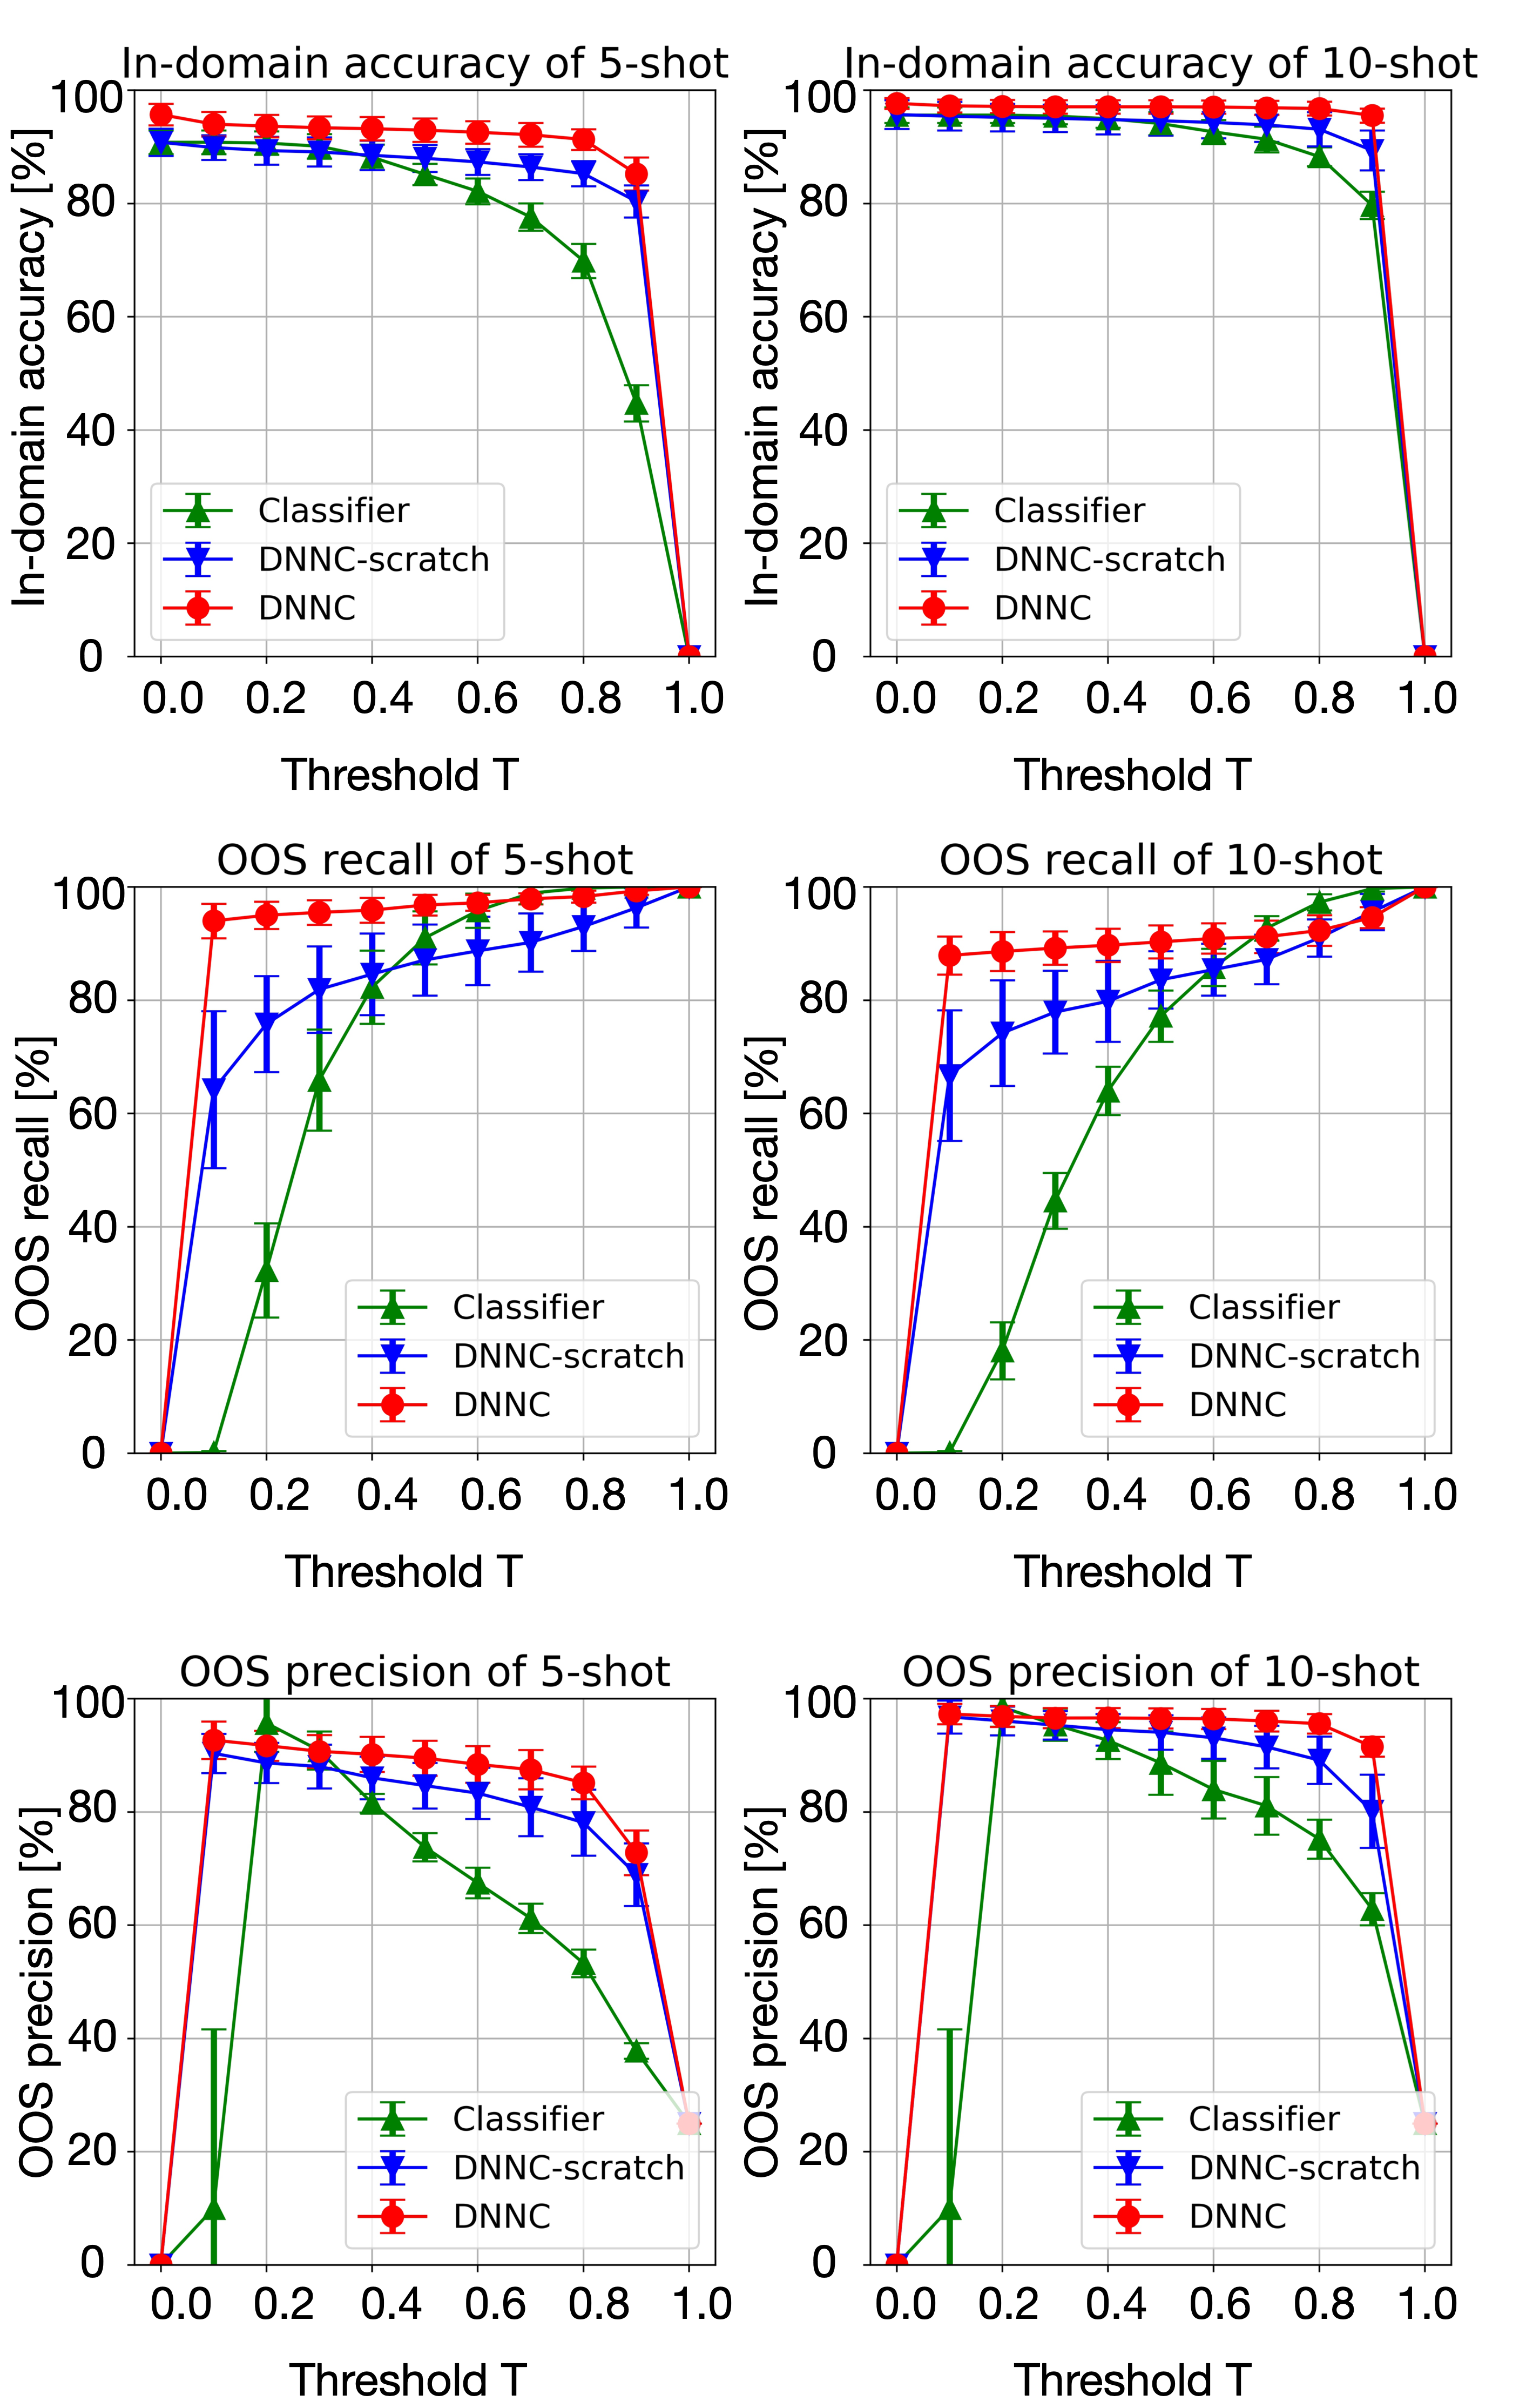
\includegraphics[width=0.85\linewidth]{./images_appendix/Visualization_Metric_Appendix.png}
    \end{center}
\caption{5-shot and 10-shot development results on the banking domain. In this series of plots, a model with a higher area-under-the-curve is more robust.}
\label{fig:visulization-appendix}
\end{figure*}

\begin{figure*}[t]
	\begin{center}
    	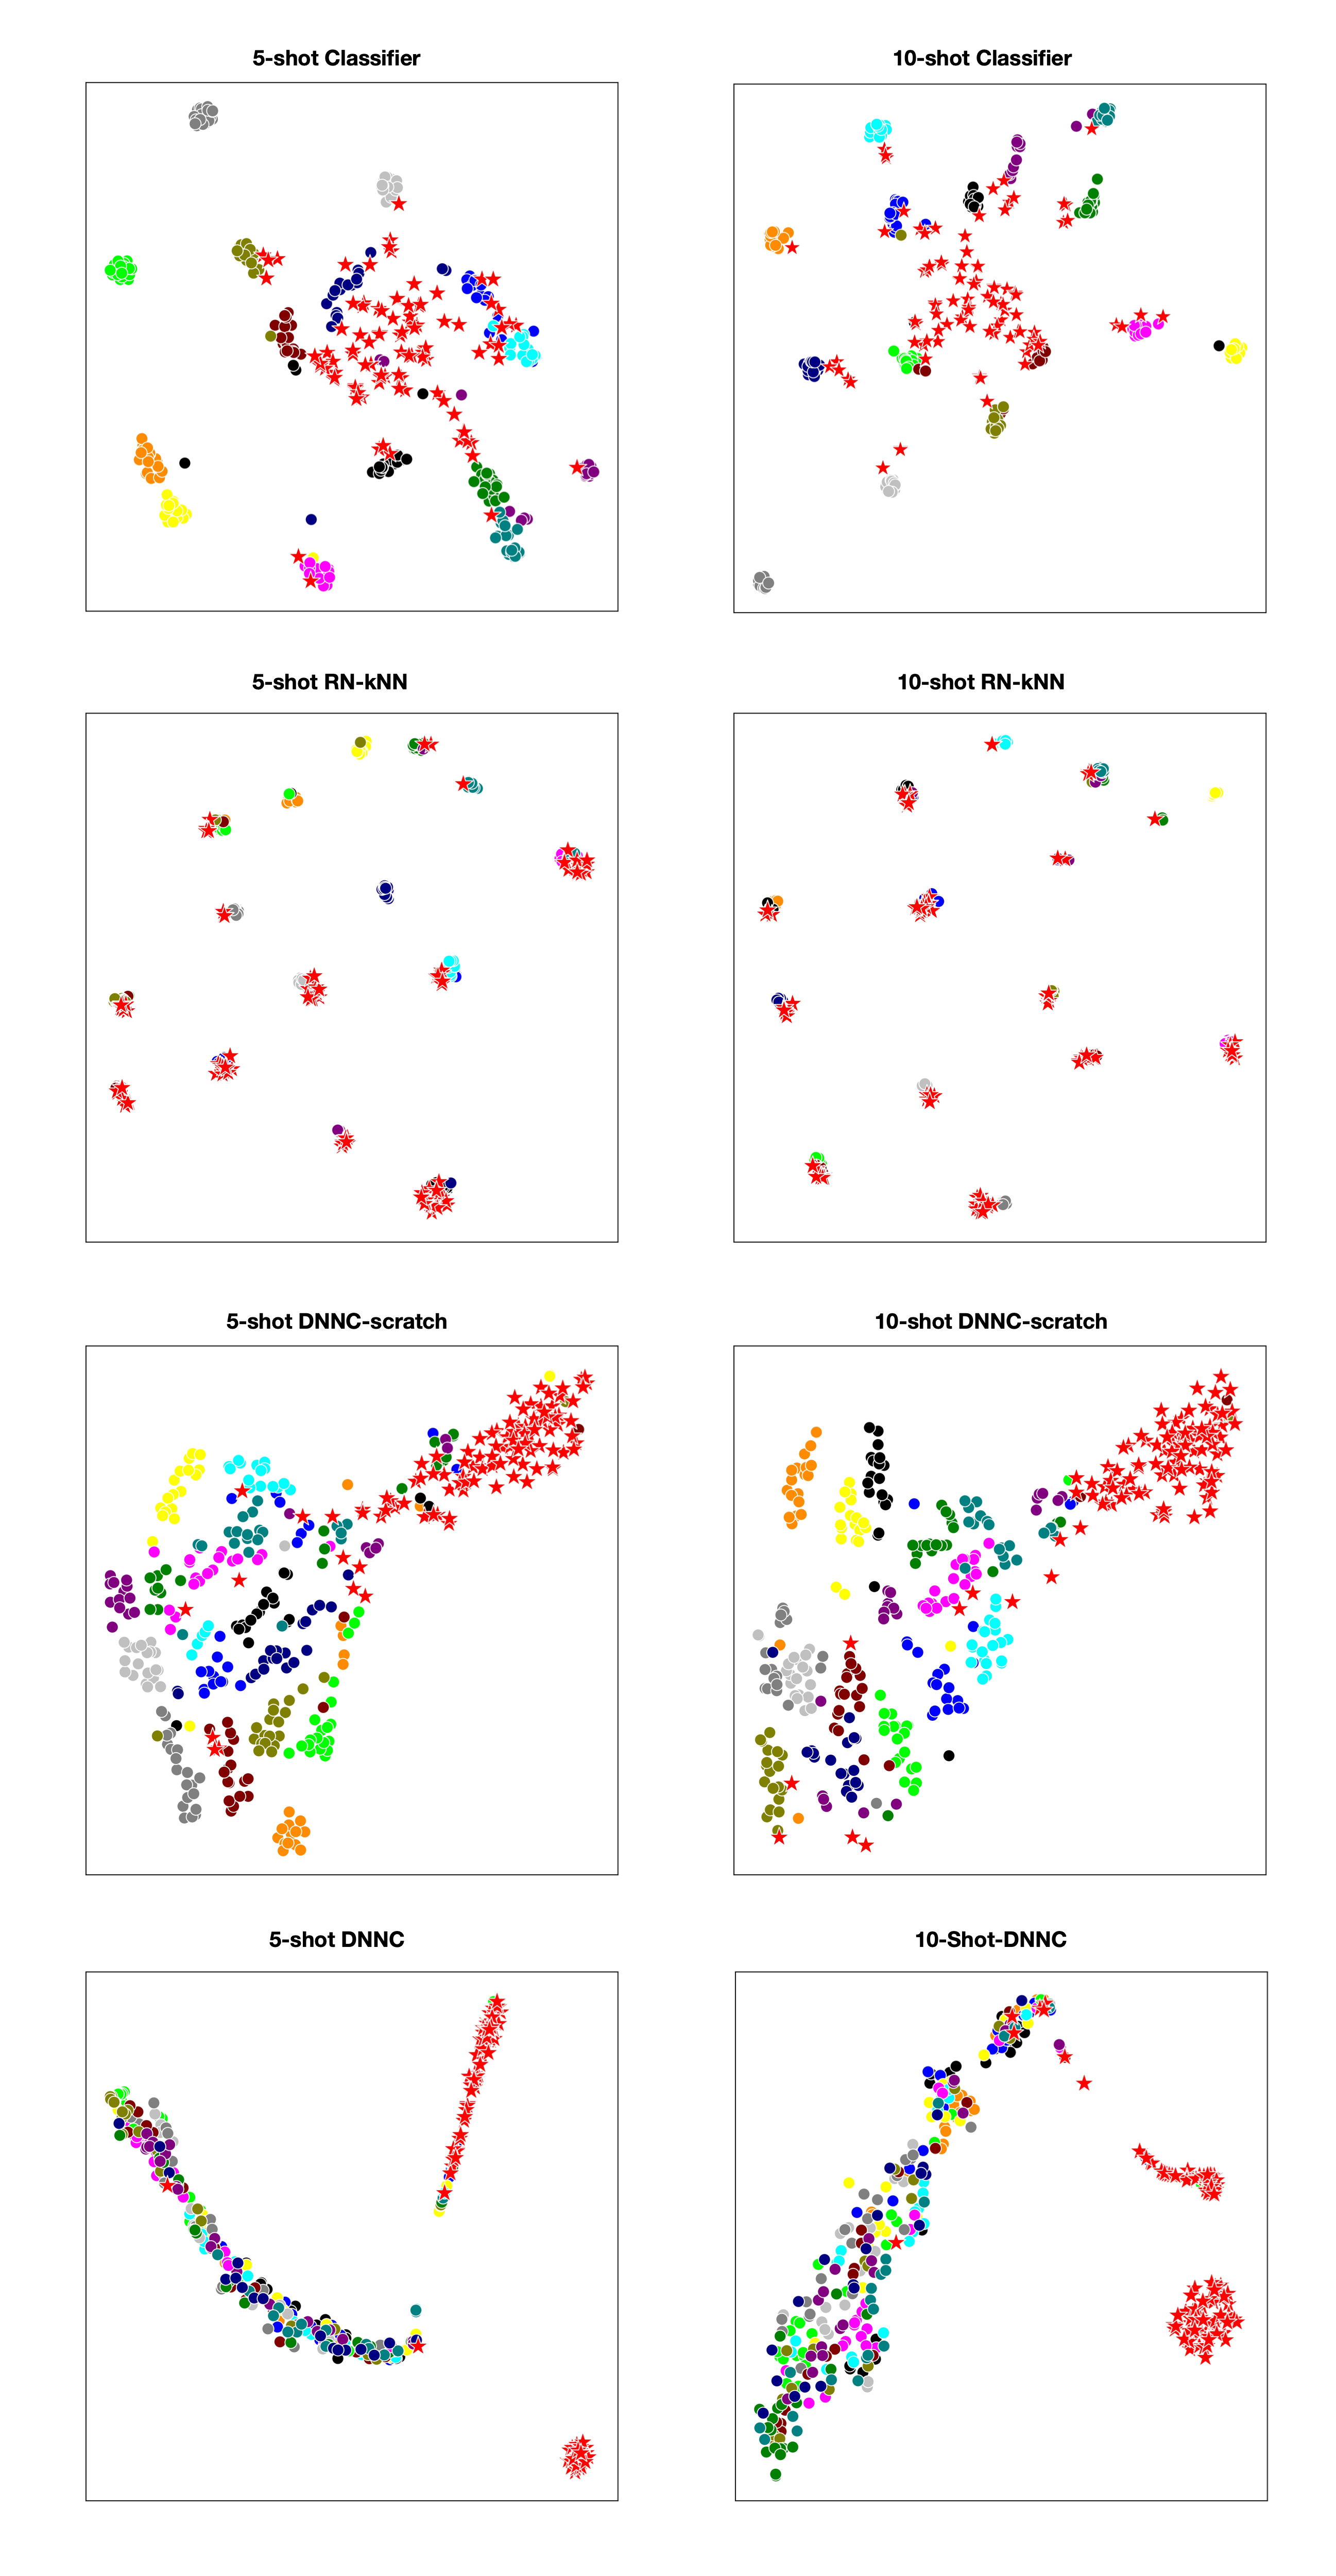
\includegraphics[width=0.85\linewidth,height=0.9\textheight]{./images_appendix/TSNE_Appendix.png}
    \end{center}
\caption{5-shot and 10-shot tSNE visualizations on development set of the banking domain, where circles represent in-domain intent classes, and red stars represent out-of-scope intents.}
\label{fig:tsne-appendix}
\end{figure*}


\begin{figure*}[t]
	\begin{center}
    	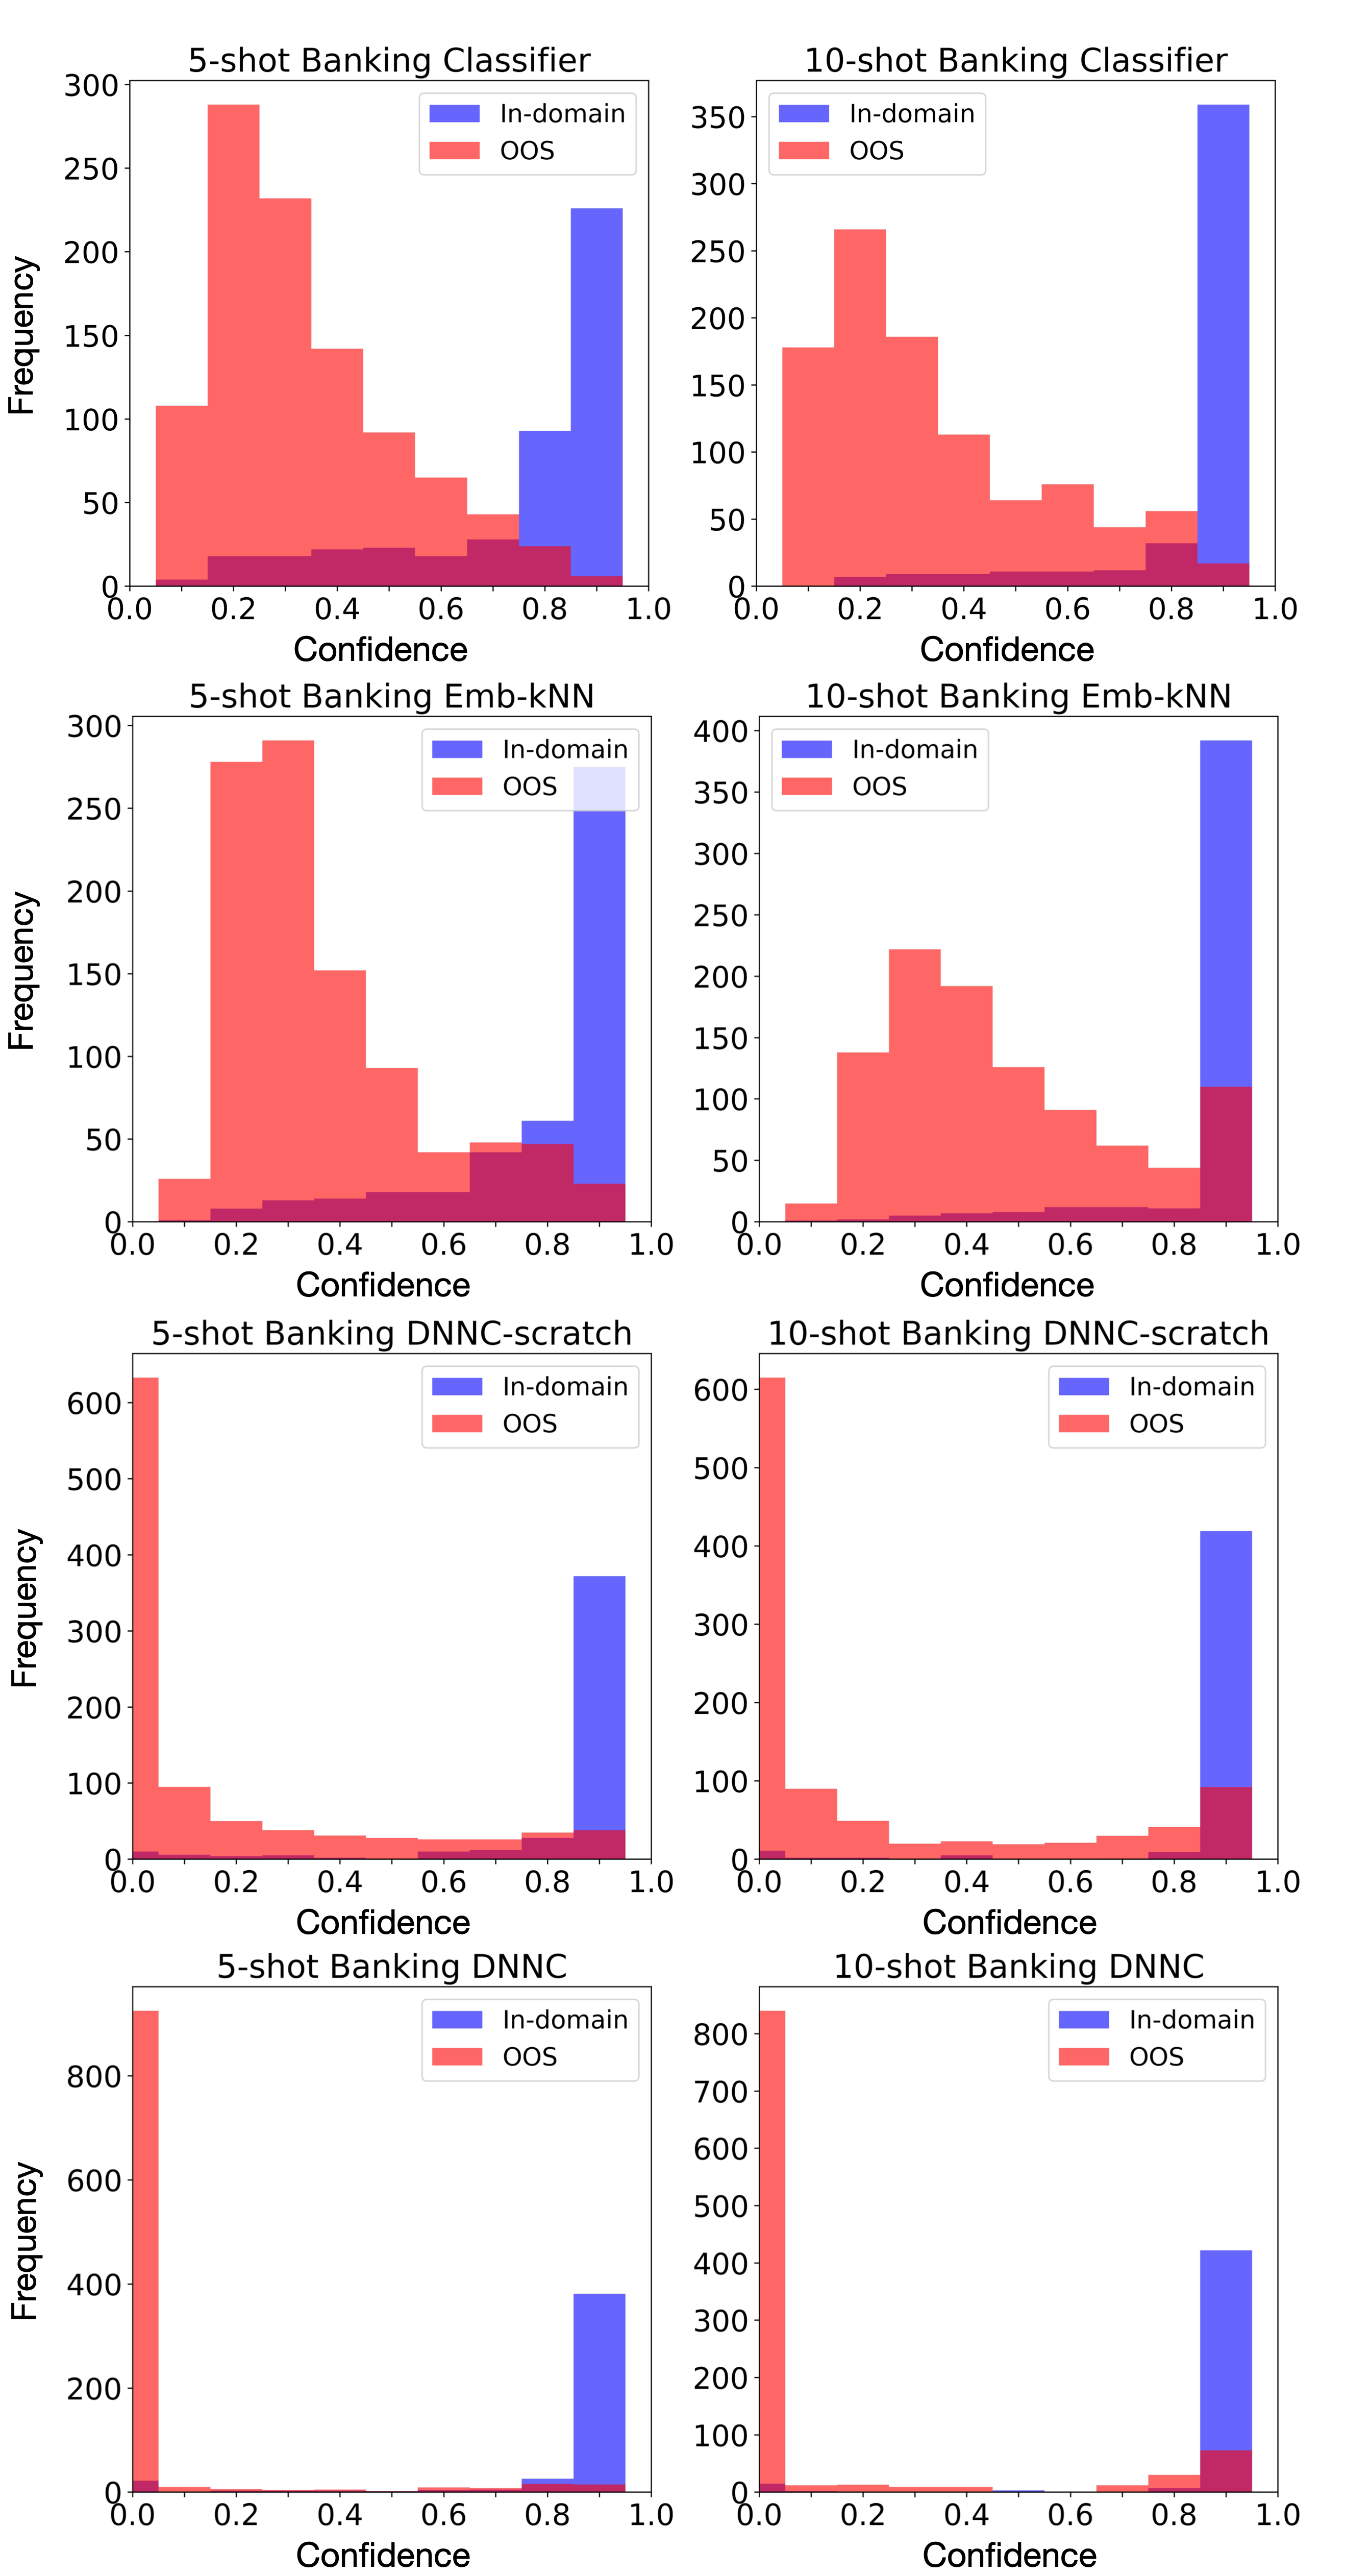
\includegraphics[width=0.85\linewidth,keepaspectratio=true,height=0.95\textheight]{./images_appendix/Conf_Appendix_with_sbert.png}
    \end{center}
\caption{5-shot and 10-shot confidence levels on test set of the banking domain. Best viewed in color.}
\label{fig:Conf-appendix}
\end{figure*}

\begin{figure*}[t]
	\begin{center}
    	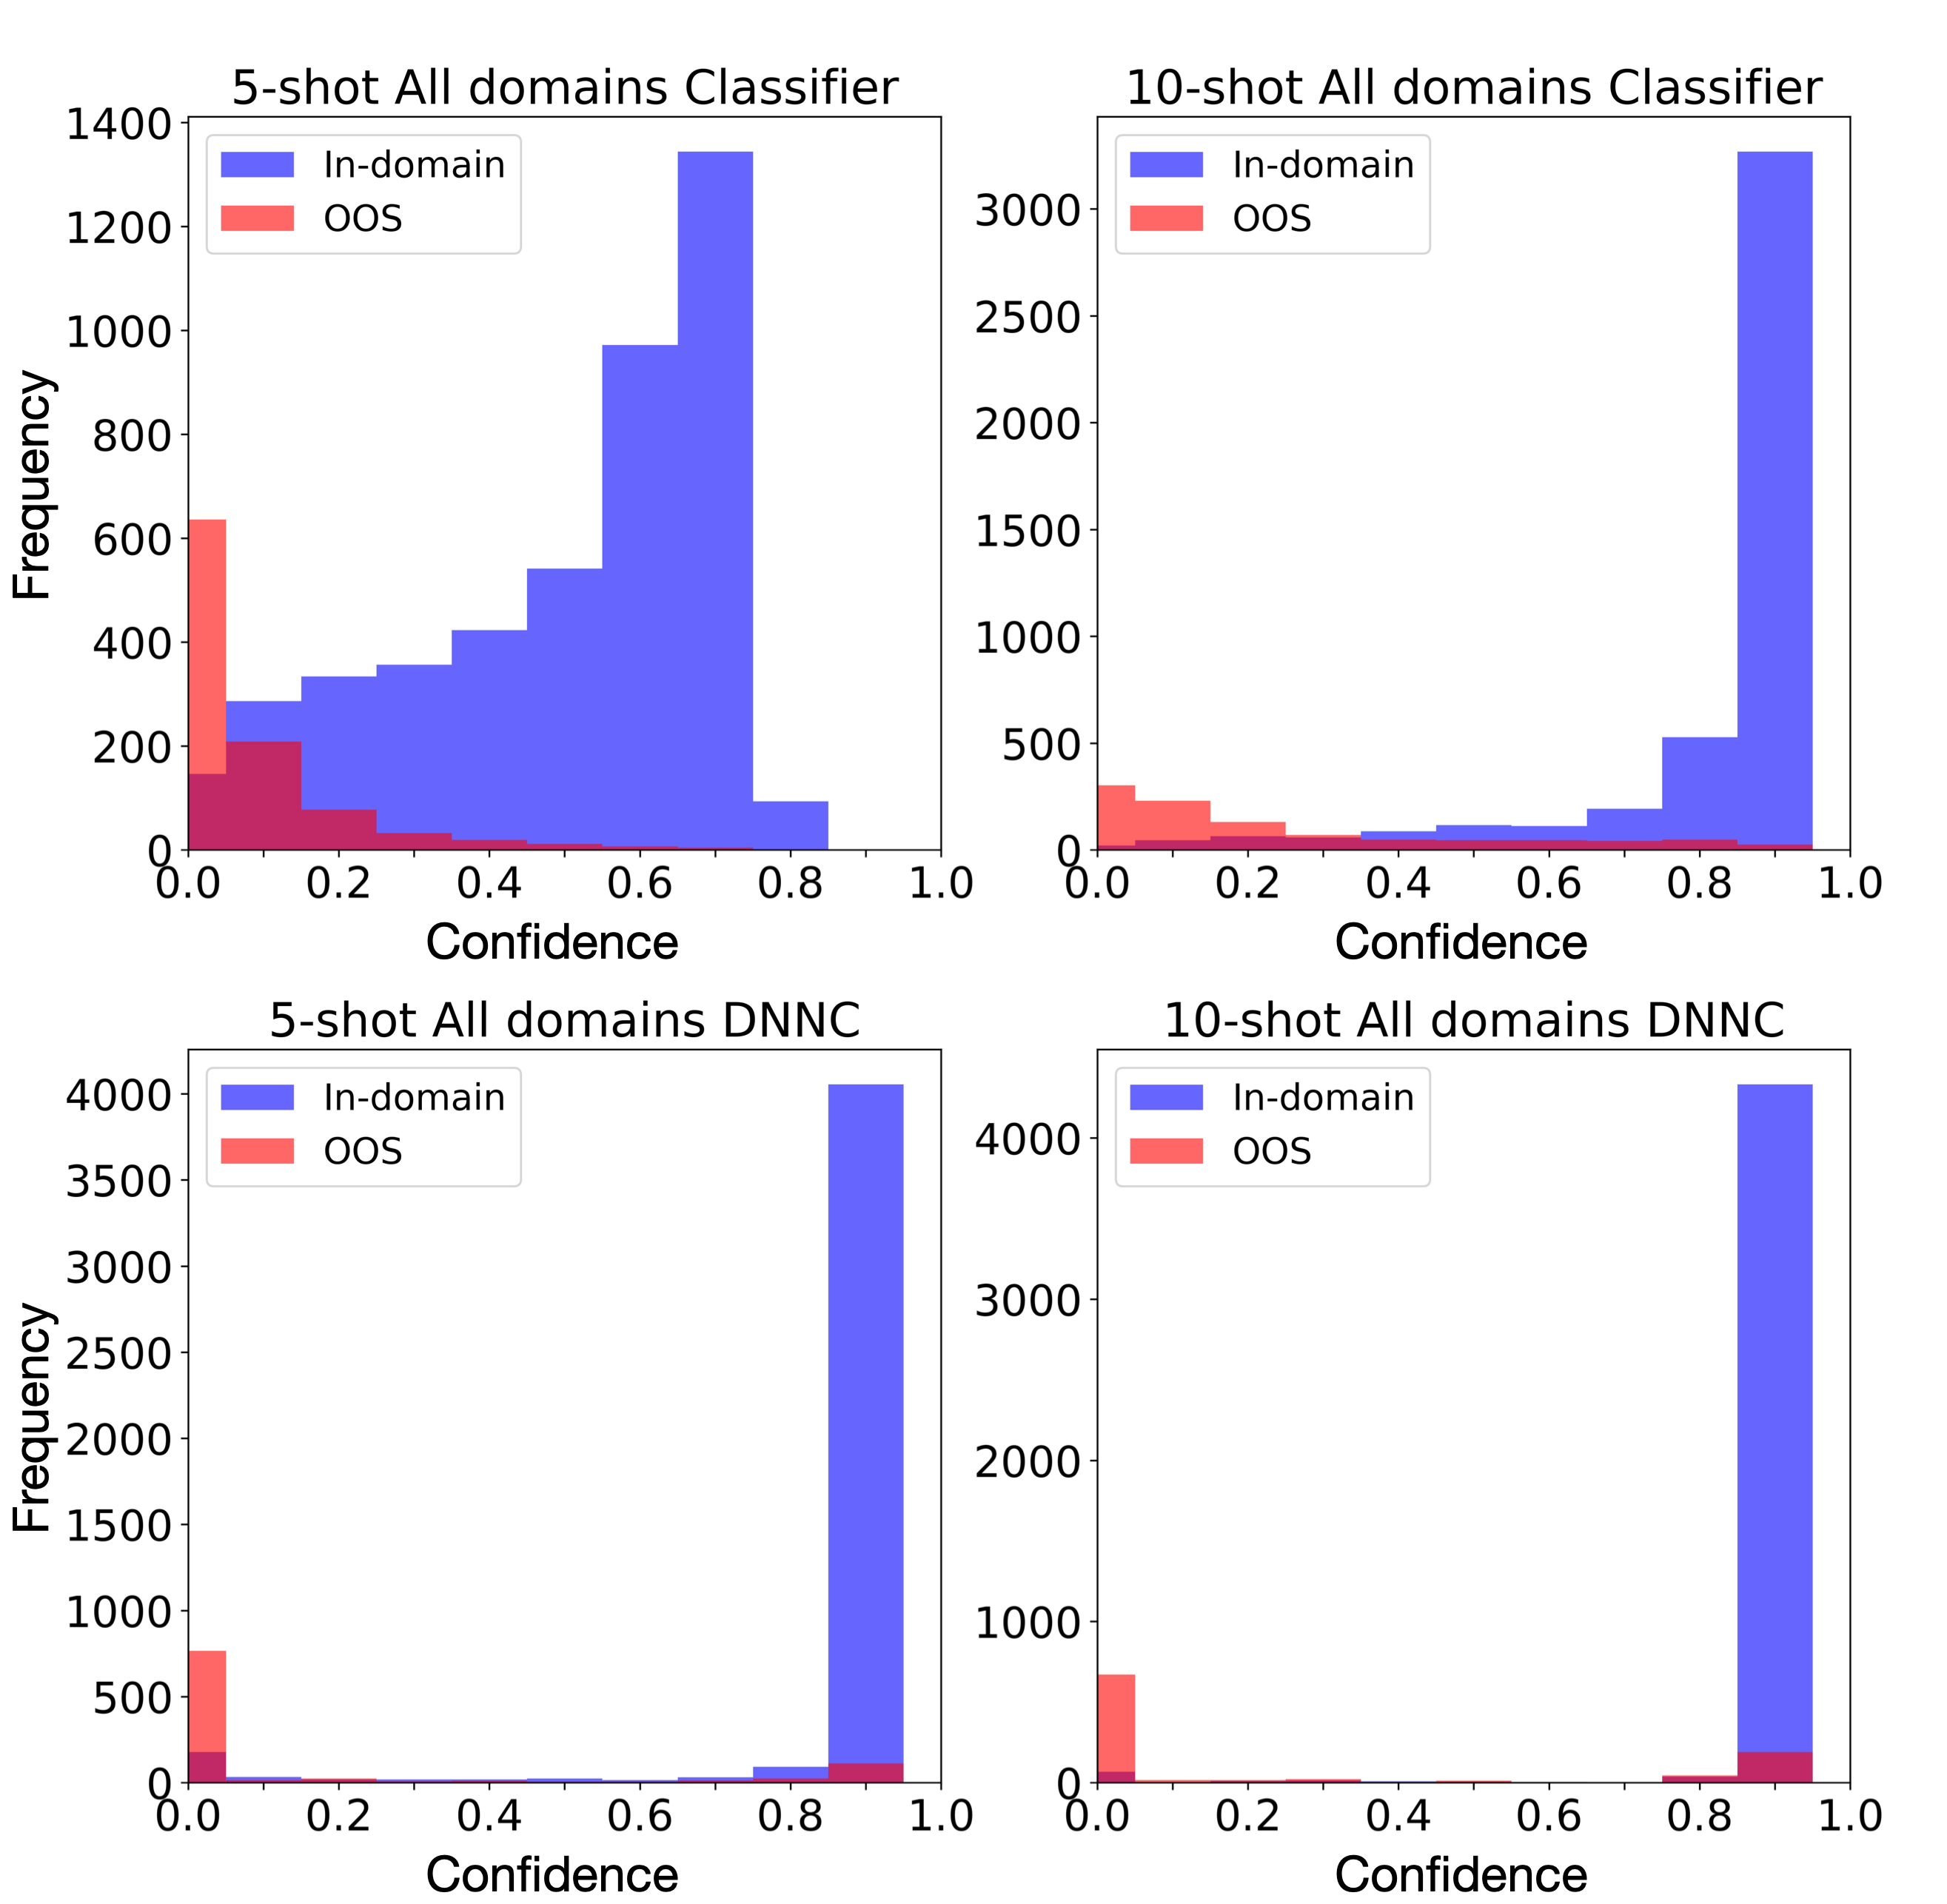
\includegraphics[width=0.85\linewidth]{./images_appendix/Conf_Appendix_All_domains.png}
    \end{center}
\caption{5-shot and 10-shot confidence levels on test set of all domains. Best viewed in color.}
\label{fig:Conf-appendix-all-domains}
\end{figure*}

\begin{figure*}[t]
	\begin{center}
    	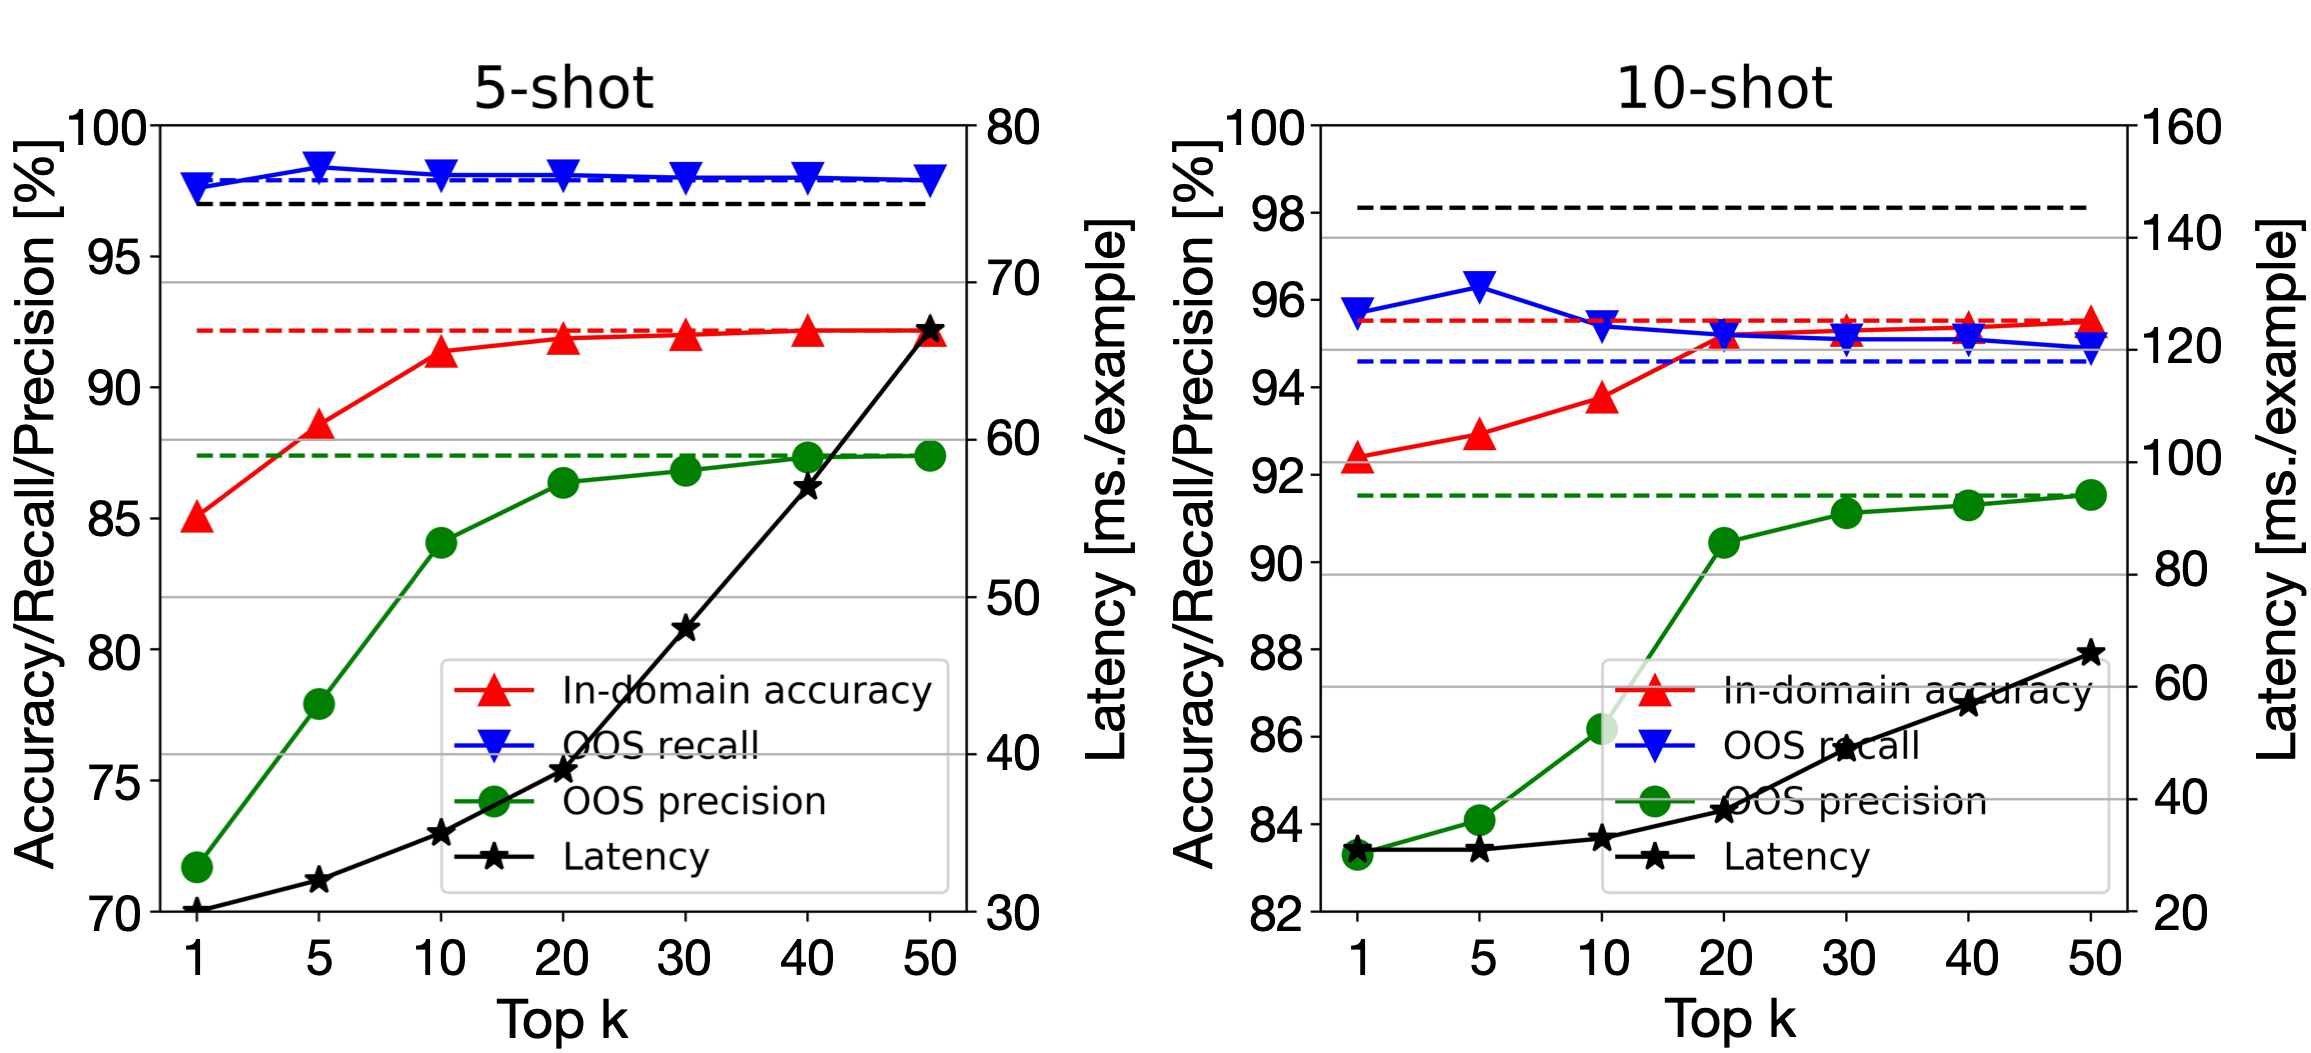
\includegraphics[width=0.85\linewidth]{./images_appendix/Visualization_Joint_nli_Appendix.png}
    \end{center}
\caption{5-shot and 10-shot DNNC-joint development results on the banking domain, where the dash lines are DNNC results.}
\label{fig:joint_nli-appendix}
\end{figure*}




